\documentclass{article}
\usepackage[T1]{fontenc}
\usepackage{garamondx}
\usepackage[garamondx,cmbraces]{newtxmath}
\usepackage{tikz}

\usetikzlibrary{positioning}
\usetikzlibrary{decorations.pathmorphing}
\usetikzlibrary{decorations.pathreplacing}
\usetikzlibrary{calc}
\usetikzlibrary{arrows}
\usetikzlibrary{automata}

\pagestyle{empty}

\begin{document}
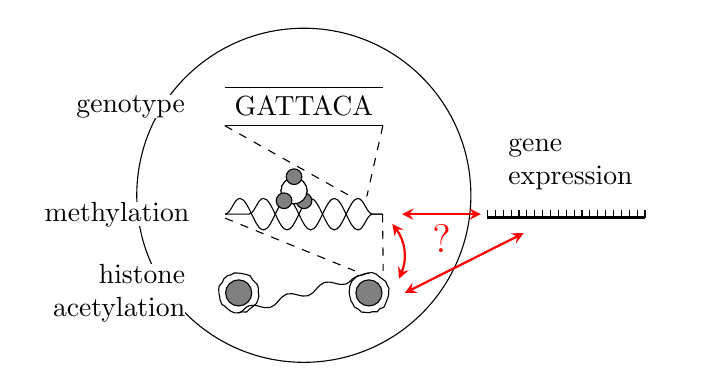
\begin{tikzpicture}
    \node (g) {GATTACA};
    \draw (g.north west) -- (g.north east);
    \draw (g.south west) -- (g.south east);

    \node [below left= of g.south] (m1) {};
    \node [below right= of g.south] (m2) {};
    \draw [decorate, decoration={snake, segment length=6mm, amplitude=2mm}] (m1) -- (m2);
    \draw [decorate, decoration={snake, segment length=6mm, amplitude=2mm, pre length=3mm}] (m1) -- (m2);
    \node [right=1cm of m1.north, anchor=south, circle, draw, fill=white] (me) { };
    \node [below right=-0.1 of me.south east, anchor=north west, circle, draw, fill=gray, inner sep=2pt] { };
    \node [right=1cm of m1.north, anchor=south, circle, draw, fill=white] (me) { };
    \node [below left=-0.1 of me.south west, anchor=north east, circle, draw, fill=gray, inner sep=2pt] { };
    \node [above=-0.1 of me.north, anchor=south, circle, draw, fill=gray, inner sep=2pt] { };

    \node [below= of m1.east, anchor=west, circle, draw, fill=gray] (a1) { };
    \node [below= of m2.west, anchor=east, circle, draw, fill=gray] (a2) { };
    \node [above=0 of a1.center, anchor=center, circle, draw, decorate,
           decoration={random steps, amplitude=0.1mm, segment length=0.5mm}, 
           inner sep=5pt] (a1out) { };
    \node [above=0 of a2.center, anchor=center, circle, draw, decorate,
           decoration={random steps, amplitude=0.1mm, segment length=0.5mm}, 
           inner sep=5pt] (a2out) { };
    \draw [decorate, decoration={snake, amplitude=0.5mm, segment length=5mm}]
          (a1out.south) -- (a2out.north);

    \draw [dashed] (g.south west) -- ($(m2.north west) + (-4mm, 1mm)$);
    \draw [dashed] (g.south east) -- ($(m2.north west) + (-2mm, 1mm)$);

    \draw [dashed] (m1) -- ($(a2out.north west) + (0mm, 1mm)$);
    \draw [dashed] (m2.west) -- ($(a2out.north east) + (0mm, 1mm)$);

    \node [circle, draw, above=of g.center, anchor=north, inner sep=1.5cm] { };

    \node [right=1cm of m2, inner sep=1pt] (e1) { };
    \node [right=2cm of e1, inner sep=1pt] (e2) { };
    \draw [decorate, decoration={ticks, amplitude=0.5mm, segment length=1mm}] (e1) -- (e2);
    \draw [thick] (e1.south east) -- (e2.south west);

    \draw [<->, >=stealth, thick, color=red] (e1) -- node [auto, color=red] {\Large{?}} (m2);
    \draw [<->, >=stealth, thick, color=red] ($(e1.south) + (5mm, -2mm)$) -- 
    ($(a2out.east) + (2mm, 0mm)$);
    \path [bend left, draw, <->, >=stealth, thick, color=red] (m2.south) to 
    ($(a2out.north east) + (2mm, 0)$);

    \node [above right=2mm of e1, text width=2cm] {gene \\ expression};
    \node [left=2mm of m1, fill=white, inner sep=0pt, align=right] {methylation};
    \node [left=5mm of a1, fill=white, inner sep=0pt, text width=2cm,
    align=right] {histone \\ acetylation};
    \node [left=5mm of g.west, fill=white, inner sep=0pt, align=right] {genotype};
\end{tikzpicture}
\end{document}
